% =====================================================================
% B.Tech Project Report (Honor/Minor) - VII Semester
% Ramdeobaba University, School of Computer Science and Engineering
%
% Project: Cloud-Based Food-Delivery Analytics Using Data Engineering
%          and Large Language Models
%
% Compiled with: pdflatex (run twice for cross-references and TOC)
%   pdflatex main.tex
%   pdflatex main.tex
%
% Placeholders still to be filled by the project team are written in
% [SQUARE BRACKETS AND ITALICS] and listed in README.md.
% =====================================================================
\documentclass[12pt,a4paper]{report}

% ---------------------------- Packages ------------------------------
\usepackage[utf8]{inputenc}
\usepackage[T1]{fontenc}
\usepackage{newtxtext,newtxmath}                 % Times New Roman
\usepackage[left=1.5in,right=1in,top=1in,bottom=1in]{geometry}
\usepackage{setspace}
\onehalfspacing                                  % 1.5 line spacing
\usepackage{amsmath}
\usepackage{titlesec}                            % heading sizes
\usepackage{fancyhdr}                            % page numbers bottom centre
\usepackage{caption}
\usepackage{booktabs}
\usepackage{array}
\usepackage{enumitem}
\usepackage[normalem]{ulem}                      % \sout for strike-outs
\usepackage{graphicx}
\usepackage{adjustbox}
\usepackage{tikz}
\usetikzlibrary{positioning,arrows.meta,shapes.geometric,fit}
\usepackage[hidelinks]{hyperref}

% Paragraph spacing: 6 pt after each paragraph (indent kept for readability)
\setlength{\parskip}{6pt plus 1pt}
\setlength{\parindent}{1.5em}
\emergencystretch=2em   % avoid margin overflows in justified text

% ------------------------- Heading formats ---------------------------
% Chapter heading: 16 pt, bold, UPPERCASE
\titleformat{\chapter}[display]
  {\centering\bfseries\fontsize{16}{20}\selectfont}
  {CHAPTER~\thechapter}
  {16pt}
  {}
\titlespacing*{\chapter}{0pt}{0pt}{30pt}
% Section heading: 14 pt, bold
\titleformat{\section}
  {\fontsize{14}{17}\selectfont\bfseries}
  {\thesection}{0.8em}{}
% Subsection heading: 12 pt, bold
\titleformat{\subsection}
  {\fontsize{12}{15}\selectfont\bfseries}
  {\thesubsection}{0.8em}{}
\renewcommand{\thesubsubsection}{\thesubsubsection.}

\captionsetup{font=small,labelfont=bf,justification=centering}

% --------------------------- Page style ------------------------------
\pagestyle{fancy}
\fancyhf{}
\fancyfoot[C]{\thepage}
\renewcommand{\headrulewidth}{0pt}
\renewcommand{\footrulewidth}{0pt}
\fancypagestyle{plain}{%
  \fancyhf{}\fancyfoot[C]{\thepage}%
  \renewcommand{\headrulewidth}{0pt}%
  \renewcommand{\footrulewidth}{0pt}}

% ----------------------- Chapter separator page ----------------------
% Separator pages carry no page number (per university guidelines)
\newcommand{\chaptersplit}[2]{%
  \clearpage
  \thispagestyle{empty}%
  \vspace*{\fill}
  \begin{center}
    {\fontsize{16}{20}\selectfont\bfseries CHAPTER #1\par}
    \vspace{1.2cm}
    {\fontsize{16}{20}\selectfont\bfseries #2\par}
  \end{center}
  \vspace*{\fill}
  \clearpage
}

% Convenience command for visible placeholders
\newcommand{\ph}[1]{\textit{[#1]}}

% TikZ styles for architecture diagrams
\tikzset{
  block/.style={draw,rounded corners,align=center,minimum height=1.1cm,
                text width=2.5cm,font=\footnotesize,fill=black!5},
  wideblock/.style={draw,rounded corners,align=center,minimum height=1.1cm,
                text width=5.2cm,font=\footnotesize,fill=black!5},
  smallblock/.style={draw,rounded corners,align=center,minimum height=0.9cm,
                text width=1.8cm,font=\scriptsize,fill=white},
  arrow/.style={-{Stealth},thick},
  darrow/.style={-{Stealth},thick,dashed},
}

\begin{document}

% =====================================================================
% 1. COVER PAGE
% =====================================================================
\begin{titlepage}
\thispagestyle{empty}
\begin{center}
{\Large\bfseries RAMDEOBABA UNIVERSITY}\\[0.3cm]
{\large School of Computer Science and Engineering}\\[0.4cm]
{\small Shri Ramdeobaba College of Engineering and Management, Nagpur}\\
{\small An Autonomous Institute affiliated to Rashtrasant Tukadoji Maharaj Nagpur University, Nagpur}\\[0.6cm]

\fbox{\parbox[c][1.8cm][c]{0.5\textwidth}{\centering\itshape [UNIVERSITY LOGO]}}\\[0.8cm]

{\large\bfseries PROJECT REPORT}\\[0.2cm]
{\normalsize B.\,Tech.\ (Honor) in Computer Science and Engineering (Data Science)\\
\sout{/\ B.\,Tech.\ (Honor) in Information Technology}}\\[0.1cm]
{\normalsize \sout{Project}\ \sout{Major Project}}\\[0.6cm]

{\normalsize ON}\\[0.5cm]

{\Large\bfseries CLOUD-BASED FOOD-DELIVERY ANALYTICS USING\\[0.15cm]
DATA ENGINEERING AND LARGE LANGUAGE MODELS}\\[1.0cm]

{\normalsize SUBMITTED BY}\\[0.3cm]
{\normalsize Amit Saw \ (Roll No.\ \_\_\_\_\_\_\_\_\_\_)\\[0.15cm]
Ankit Kolhe \ (Roll No.\ \_\_\_\_\_\_\_\_\_\_)\\[0.15cm]
Aryan Paradkar \ (Roll No.\ \_\_\_\_\_\_\_\_\_\_)}\\[0.3cm]
{\normalsize OF VII SEMESTER}\\[0.8cm]

{\normalsize UNDER THE GUIDANCE OF}\\[0.2cm]
{\normalsize\bfseries Prof.\,/\,Dr.\ [Guide Name]}\\[0.1cm]
{\small Project Guide, Department of Computer Science and Engineering}\\[1.0cm]

{\normalsize ACADEMIC YEAR: 2026--2027}
\end{center}
\end{titlepage}

\pagenumbering{roman}
\setcounter{page}{2}   % cover = page i (number not printed)

% =====================================================================
% 2. CERTIFICATE
% =====================================================================
\chapter*{CERTIFICATE}
\addcontentsline{toc}{chapter}{CERTIFICATE}
\begin{center}
{\small SHRI RAMDEOBABA COLLEGE OF ENGINEERING AND MANAGEMENT, NAGPUR}\\[0.1cm]
{\small (An Autonomous Institute affiliated to Rashtrasant Tukadoji Maharaj Nagpur University, Nagpur)}\\[0.1cm]
{\small DEPARTMENT OF COMPUTER SCIENCE AND ENGINEERING}\\[1.5cm]
{\Large\bfseries CERTIFICATE}
\end{center}

\vspace{0.8cm}
\noindent This is to certify that the Project Report on ``Cloud-Based Food-Delivery Analytics Using Data Engineering and Large Language Models'' is a bonafide work of Amit Saw, Ankit Kolhe and Aryan Paradkar, submitted to the Rashtrasant Tukadoji Maharaj Nagpur University, Nagpur in partial fulfilment of the award of the Degree of Bachelor of Technology (B.\,Tech.) (Honor) in Computer Science and Engineering (Data Science) / Information Technology. It has been carried out at the Department of Computer Science and Engineering, Shri Ramdeobaba College of Engineering and Management, Nagpur during the academic year 2026--2027.

\vspace{1.5cm}
\noindent Date:\ \_\_\_\_\_\_\_\_\_\_\_\_\_\_\_\_\_\_\_ \hfill Place: Nagpur

\vspace{2.0cm}
\begin{tabular}{@{}p{0.45\textwidth}p{0.45\textwidth}@{}}
\rule{6.5cm}{0.4pt} & \rule{6.5cm}{0.4pt} \\
Name of Guide & External Examiner \\
Project Guide &  \\[1.2cm]
\rule{6.5cm}{0.4pt} & \rule{6.5cm}{0.4pt} \\
Dr.\ A.\ M.\ Karandikar & Dr.\ M.\ B.\ Chandak \\
Associate Head & Principal \\
Department of Computer Science \& Engineering & \\
\end{tabular}

% =====================================================================
% 3. STUDENT DECLARATION
% =====================================================================
\chapter*{STUDENT DECLARATION}
\addcontentsline{toc}{chapter}{STUDENT DECLARATION}

\noindent We hereby declare that the project report entitled ``Cloud-Based Food-Delivery Analytics Using Data Engineering and Large Language Models'' is submitted as part of the requirements for the B.\,Tech.\ (Honor) in Computer Science and Engineering (Data Science) / Information Technology programme at Ramdeobaba University.

The work presented in this report is prepared by the undersigned students under the guidance of the project supervisor. All external sources, datasets, software tools, figures and technical material used in the project have been appropriately acknowledged. Where measured values were not available at the time of submission, the report contains clearly marked placeholders; these indicate measurements that are to be recorded from actual runs, and no unmeasured results are claimed as final.

\vspace{1.5cm}
\noindent Amit Saw \ \rule{5cm}{0.4pt} \ (Roll No.\ \_\_\_\_\_\_\_\_\_\_)

\vspace{0.6cm}
\noindent Ankit Kolhe \ \rule{5cm}{0.4pt} \ (Roll No.\ \_\_\_\_\_\_\_\_\_\_)

\vspace{0.6cm}
\noindent Aryan Paradkar \ \rule{5cm}{0.4pt} \ (Roll No.\ \_\_\_\_\_\_\_\_\_\_)

% =====================================================================
% 4. APPROVAL SHEET
% =====================================================================
\chapter*{APPROVAL SHEET}

\noindent This report entitled ``Cloud-Based Food-Delivery Analytics Using Data Engineering and Large Language Models'' by Amit Saw, Ankit Kolhe and Aryan Paradkar is approved for the degree of Bachelor of Technology (B.\,Tech.) (Honor) in Computer Science and Engineering (Data Science) / Information Technology.

\vspace{1.5cm}
\begin{tabular}{@{}p{0.45\textwidth}p{0.45\textwidth}@{}}
\rule{6.5cm}{0.4pt} & \rule{6.5cm}{0.4pt} \\
Name of Guide & External Examiner \\
Project Guide &  \\[1.5cm]
\rule{6.5cm}{0.4pt} \\
Dr.\ A.\ M.\ Karandikar \\
Associate Head, CSE & \\
\end{tabular}

\vspace{1.0cm}
\noindent Date:\ \_\_\_\_\_\_\_\_\_\_\_\_\_\_\_\_\_\_\_ \hfill Place: Nagpur

% =====================================================================
% 5. ACKNOWLEDGEMENT
% =====================================================================
\chapter*{ACKNOWLEDGEMENT}
\addcontentsline{toc}{chapter}{ACKNOWLEDGEMENT}

\noindent We express our sincere gratitude to Ramdeobaba University and the School of Computer Science and Engineering for providing the academic environment and facilities required to complete this project.

We are grateful to our project guide, Prof.\,/\,Dr.\ [Guide Name], for continuous guidance, technical suggestions and constructive feedback throughout the project. We also thank the Project In-Charge, Associate Head and Dean, School of Computer Science and Engineering, for their support.

We acknowledge the support of our classmates, laboratory staff, friends and family members who contributed directly or indirectly to the completion of this work. We also thank the open-source and documentation communities of Amazon Web Services, Snowflake, dbt Labs, Apache Software Foundation, Streamlit and xAI, whose resources made the implementation of this prototype possible.

% =====================================================================
% 6. ABSTRACT
% =====================================================================
\chapter*{ABSTRACT}
\addcontentsline{toc}{chapter}{ABSTRACT}

\noindent Food-delivery platforms produce two very different kinds of data. Structured records such as orders, order items, restaurants, customers and menu items describe what happened in the business, while free-form customer reviews describe how customers experienced the food, service, pricing and delivery. These data sources provide complementary insight, but they are frequently processed in separate workflows, which makes it difficult to connect operational performance with the reasons customers report in their feedback.

This report presents the design and implementation of a cloud-based analytics prototype that combines a layered data pipeline with large language model (LLM) assisted access to business information. The pipeline uses Amazon S3~\cite{ref20} for raw-file storage, Snowflake~\cite{ref21} as the analytical warehouse organised into Bronze, Silver and Gold layers, dbt for declarative SQL transformations and data-quality testing, and Apache Airflow for workflow orchestration. A Streamlit~\cite{ref22} interface supports two forms of interaction: review analysis, in which selected review text and a user instruction are sent to the Grok API, and natural-language-to-SQL querying, in which a question about the business is translated into a read-only query over curated analytical tables.

Because the review module uses direct prompting rather than a labelled classification pipeline or an embedding-based retrieval system, the report deliberately makes no claim of classification accuracy or retrieval quality. Evaluation is framed as pipeline checks, data-quality test outcomes, Text-to-SQL execution checks, qualitative inspection of review answers and operational observations. The contribution of the work is the integrated system design, the guardrails around natural-language database access, and a repeatable evaluation methodology into which measured results can be inserted.

\vspace{0.4cm}
\noindent\textbf{Keywords:} Cloud Data Engineering, Food-Delivery Analytics, Snowflake, dbt, Apache Airflow, Large Language Models, Natural-Language Querying, Streamlit

% =====================================================================
% 7-9. TOC, LIST OF FIGURES, LIST OF TABLES
% =====================================================================
\clearpage
\tableofcontents

\clearpage
\addcontentsline{toc}{chapter}{LIST OF FIGURES}
\listoffigures

\clearpage
\addcontentsline{toc}{chapter}{LIST OF TABLES}
\listoftables

% =====================================================================
% 10. LIST OF ABBREVIATIONS
% =====================================================================
\clearpage
\chapter*{LIST OF ABBREVIATIONS}
\addcontentsline{toc}{chapter}{LIST OF ABBREVIATIONS}

\begin{center}
\begin{tabular}{@{}ll@{}}
\toprule
\textbf{Abbreviation} & \textbf{Meaning} \\
\midrule
AI & Artificial Intelligence \\
API & Application Programming Interface \\
ACID & Atomicity, Consistency, Isolation, Durability \\
CSV & Comma-Separated Values \\
DAG & Directed Acyclic Graph \\
dbt & Data Build Tool \\
ELT & Extract, Load, Transform \\
JSON & JavaScript Object Notation \\
LLM & Large Language Model \\
ML & Machine Learning \\
NL-to-SQL & Natural Language to Structured Query Language \\
RAG & Retrieval-Augmented Generation \\
REST & Representational State Transfer \\
S3 & Amazon Simple Storage Service \\
SQL & Structured Query Language \\
UI & User Interface \\
URL & Uniform Resource Locator \\
\bottomrule
\end{tabular}
\end{center}

% =====================================================================
% CHAPTER 1: INTRODUCTION
% =====================================================================
\clearpage
\pagenumbering{arabic}   % Arabic page numbers from Chapter 1 onwards

\chaptersplit{1}{INTRODUCTION}

\chapter{INTRODUCTION}

\noindent Food-delivery systems operate as multi-sided marketplaces in which customers, restaurants and delivery partners interact through a digital platform. Every interaction leaves a data trail: orders and order items record transactions, restaurant and customer tables record entities and preferences, and reviews record free-form opinions about food quality, delivery time, pricing and service. Individually, each stream is useful; together they can explain not only what is happening in a business but also why customers perceive it that way.

\noindent This chapter introduces the domain, states the problem addressed by the project, lists the objectives, defines the scope of the prototype and describes the organisation of the remainder of the report.

\section{Background}
Modern analytical architectures increasingly separate storage from transformation and organise data into layered models to improve reliability and reuse. Lakehouse research highlights the value of combining flexible object storage with structured warehouse-style processing~\cite{ref1}, and surveys of data-engineering tooling describe a mature ecosystem covering ingestion, transformation and orchestration~\cite{ref2}. At the same time, Transformer-based language models~\cite{ref3} and large language models~\cite{ref4} have made it practical to interact with text and data through natural language. Retrieval-augmented generation~\cite{ref5} and Text-to-SQL research such as the Spider dataset~\cite{ref6} have further expanded what non-specialist users can ask of a system.

These developments make it practical to design a single workflow in which raw delivery data is retained verbatim, transformed into tested analytical models, and then consumed by applications that mix dashboards, review summarisation and natural-language database access. This project focuses on that integration boundary between data engineering and AI-assisted analytics rather than on proposing a new language model. Data handling is performed in Python with the Pandas library~\cite{ref24}, and review analysis is performed through the Grok API~\cite{ref23}.

\section{Problem Statement}
In many prototype and educational analytics systems, operational records and customer reviews are handled in separate pipelines. This creates three practical limitations. First, it is difficult to link operational metrics such as delivery time or order value with the qualitative reasons customers report in reviews. Second, repeated loading, cleaning and analysis steps are performed manually, which is slow and error-prone. Third, business stakeholders who do not know SQL depend on technical staff for even routine questions.

The problem addressed in this project is therefore the design and implementation of a unified, layered cloud analytics prototype that ingests food-delivery data, curates it into tested analytical models, and exposes both structured metrics and review-derived insights through simple natural-language interfaces.

\section{Objectives}
The main objective is to build a single analytics prototype that connects cloud data processing with AI-assisted access to business information and customer feedback. The work is divided into the following objectives:
\begin{itemize}[leftmargin=2em]
\item To collect and store food-delivery data, including orders, customers, restaurants, menu items and customer reviews.
\item To organise data into Bronze, Silver and Gold layers so that raw, cleaned and business-ready data remain separate.
\item To use dbt to define transformations and run data-quality checks on analytical models.
\item To use Apache Airflow to schedule and coordinate the data-pipeline tasks.
\item To send selected review text to the Grok API so users can request summaries, common themes and review-based observations.
\item To support natural-language questions over approved business tables by generating and executing read-only SQL queries.
\item To present results through a Streamlit interface that is understandable to technical and non-technical users.
\end{itemize}

\section{Scope}
The project covers data acquisition, storage, layered transformation, data-quality testing, workflow orchestration, AI-assisted review analysis, natural-language querying and visualisation. The prototype is intended for academic and engineering demonstration on a provided dataset; it does not handle live orders, real payments or production customer accounts.

The review feature performs direct LLM-based analysis of supplied review text; it does not implement embedding-based retrieval and is not a validated sentiment classifier. Similarly, the Text-to-SQL feature is a guarded prototype, not a production database interface. Claims about accuracy, time savings or business improvement are made only where those outcomes have actually been measured and recorded.

\section{Organisation of the Report}
Chapter~1 introduces the problem and objectives. Chapter~2 presents the literature review and research gap. Chapter~3 describes the proposed system and methodology. Chapter~4 discusses system design and implementation. Chapter~5 presents results and discussion. Chapter~6 concludes the work and presents future scope. The references, an appendix of configurations and prompt templates, and three annexures follow the chapters.

% =====================================================================
% CHAPTER 2: LITERATURE REVIEW AND RESEARCH GAP
% =====================================================================
\chaptersplit{2}{LITERATURE REVIEW AND RESEARCH GAP}

\chapter{LITERATURE REVIEW AND RESEARCH GAP}

\noindent The literature review establishes the technical context of the proposed system by examining cloud data architectures, data-engineering tooling, language models and retrieval methods, sentiment analysis of reviews, and Text-to-SQL research. The review is used to justify the methodology adopted in Chapter~3 and to identify the gap this project addresses.

\section{Introduction}
Research relevant to this project falls into five themes: (i) cloud data platforms and lakehouse architectures; (ii) data-engineering pipeline tooling; (iii) language models and retrieval-augmented generation; (iv) sentiment and opinion analysis of restaurant and delivery reviews; and (v) natural-language database interfaces. Each theme is reviewed below, followed by a comparison of representative approaches and a statement of the research gap.

\section{Review of Existing Approaches}

\subsection{Cloud Data Platforms and Lakehouse Architectures}
Lakehouse research examines ways to bring data-lake flexibility and warehouse-style management into a common analytical architecture~\cite{ref1,ref7}. The Delta Lake work demonstrates that ACID table storage can be built over cloud object stores, which makes layered batch pipelines practical without a traditional warehouse-only design~\cite{ref8}. For this project, the relevant lesson is architectural: raw data and curated analytical data have different purposes and should be managed deliberately, as separate layers rather than as one overwritten table.

\subsection{Data-Engineering Pipeline Tooling}
A survey of pipeline tools for data engineering~\cite{ref2} describes the distinct roles of ingestion, transformation and orchestration in reliable workflows, and production machine-learning experience shows that data management, not model code, dominates pipeline effort~\cite{ref9}. Frameworks such as dbt~\cite{ref19} make transformations explicit, testable SQL models, while Apache Airflow~\cite{ref18} sequences and schedules them as directed acyclic graphs. These ideas inform the decision to treat S3, Snowflake, dbt and Airflow as distinct components rather than collapsing the pipeline into one script.

\subsection{Language Models and Retrieval-Augmented Generation}
The Transformer architecture~\cite{ref3} underpins modern large language models, whose few-shot capabilities~\cite{ref4} allow a user instruction and a block of supplied text to produce useful analysis without task-specific training. Retrieval-augmented generation (RAG) describes methods that provide language models with external evidence at response time~\cite{ref5}, and surveys trace its evolution and current landscape~\cite{ref10}. General LLM surveys provide broader context on capabilities and limitations~\cite{ref13}. The current review module differs from a retrieval-augmented design: review text is supplied directly to the Grok API prompt and the answer is generated from that provided context, so this report describes it as direct LLM-based review analysis, not as a vector-search RAG implementation.

\subsection{Sentiment and Opinion Analysis of Reviews}
Work on sentiment analysis of restaurant reviews shows that Transformer models can be applied to review text, including in resource-constrained edge settings~\cite{ref11}, and bidirectional pre-training remains a standard baseline~\cite{ref12}. Such studies typically require labelled training or evaluation data. Because this project has no labelled review dataset, conventional sentiment-classification accuracy is not claimed; the review module is evaluated by qualitative inspection of its answers instead.

\subsection{Natural-Language Database Interfaces (Text-to-SQL)}
Text-to-SQL research has produced large labelled benchmarks such as Spider~\cite{ref6}, large-scale database-grounded evaluation such as BIRD~\cite{ref14}, and schema-aware synthesis methods such as CHESS~\cite{ref15}. Earlier work includes reinforcement-learning query generation~\cite{ref16} and table pre-training~\cite{ref17}. These studies show both the promise and the difficulty of translating questions into valid SQL over real databases, and they motivate providing the model with a limited schema description and restricting the generated query path. They do not establish that a student prototype reaches benchmark accuracy; such a claim would require a defined test set and measured results.

\section{Comparison of Existing Approaches}
Table~\ref{tab:lit} compares representative existing approaches along their data source, main technique and typical limitation.

\begin{table}[htbp]
\centering
\caption{Comparison of representative existing approaches}
\label{tab:lit}
\small
\begin{tabular}{@{}p{3.1cm}p{2.6cm}p{3.4cm}p{4.2cm}@{}}
\toprule
\textbf{Approach} & \textbf{Data Source} & \textbf{Main Technique} & \textbf{Typical Limitation} \\
\midrule
Lakehouse platforms~\cite{ref1,ref7,ref8} & Cloud object stores & Unified batch and table storage & No built-in natural-language access \\
Pipeline tooling surveys~\cite{ref2,ref9} & Mixed sources & Ingestion, transformation, orchestration & Tool-centric; AI access left to separate systems \\
Sentiment analysis of reviews~\cite{ref11,ref12} & Labelled review corpora & Trained classifier & Requires labelled training data \\
RAG systems~\cite{ref5,ref10} & External document stores & Retrieval plus generation & Requires retrieval infrastructure and indexing \\
Text-to-SQL research~\cite{ref6,ref14,ref15} & Schemas and questions & Schema linking and SQL synthesis & Benchmark accuracy does not transfer automatically \\
Dashboard / BI tools & Stored measurements & Visualisation & Business users still need SQL or report authors \\
\bottomrule
\end{tabular}
\end{table}

\section{Limitations of Existing Work}
The reviewed approaches can involve challenges related to heterogeneous data sources, inconsistent sampling intervals, data quality, communication reliability and integration between monitoring and analytics. Dashboard systems may present measurements without analytical summaries, while LLM-based tools may present fluent answers without a reliable data foundation. Text-to-SQL systems can generate syntactically valid queries that still answer the wrong question, and keyword-level safety checks alone are not a sufficient security boundary. Sending review text to an external API additionally raises data-governance, cost and rate-limit concerns that purely internal pipelines do not face.

\section{Research Gap}
The research gap addressed by this project is the integration of layered cloud data processing, declarative transformation with automated data-quality tests, workflow orchestration, direct LLM review analysis and guarded natural-language database access in one lightweight, campus-demonstrable system. Existing work generally solves one or two of these problems well, but a single reference implementation that keeps raw, cleaned and business-ready data separate while offering both structured and unstructured natural-language interaction is not commonly available for the food-delivery domain. This project contributes such an integrated prototype together with an honest evaluation methodology.

% =====================================================================
% CHAPTER 3: PROPOSED SYSTEM AND METHODOLOGY
% =====================================================================
\chaptersplit{3}{PROPOSED SYSTEM AND METHODOLOGY}

\chapter{PROPOSED SYSTEM AND METHODOLOGY}

\noindent The proposed system consists of five components: ingestion, storage, transformation and quality, AI services, and presentation. Raw files are collected and loaded into cloud object storage, curated into layered warehouse tables, tested declaratively, orchestrated by a scheduler, and finally exposed through a single web interface that supports dashboards, review analysis and natural-language querying.

\section{Proposed System}
Figure~\ref{fig:arch} shows the overall architecture. Source files for customers, restaurants, menu items, orders, order items and reviews are uploaded to Amazon S3 and loaded into Snowflake, where the Bronze layer keeps the raw representation. dbt models clean and standardise the data into Silver tables and build curated Gold dimensions, facts and business marts. Data-quality tests run as part of the transformation step. Apache Airflow coordinates the sequence and schedules repeat runs. From the Gold layer, the Streamlit application serves dashboard metrics and the natural-language-to-SQL feature, while the review-analysis feature sends selected review text to the Grok API.

\begin{figure}[htbp]
\centering
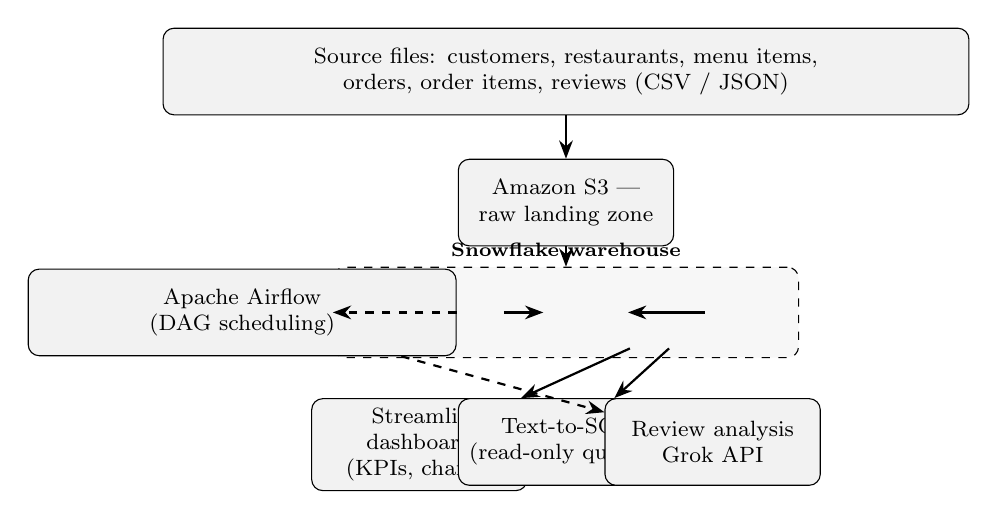
\begin{tikzpicture}[node distance=0.55cm and 0.6cm]
\node[block,text width=10cm] (src) {Source files: customers, restaurants, menu items, orders, order items, reviews (CSV / JSON)};
\node[block,below=of src] (s3) {Amazon S3 --- raw landing zone};
\node[draw,rounded corners,fill=black!3,inner sep=8pt,below=of s3] (snow) {};
\node[smallblock,left=0.5cm of snow] (brz) {Bronze\\(raw copy)};
\node[smallblock,right=0.5cm of snow] (gld) {Gold\\(marts)};
\node[smallblock,right=0.5cm of brz] (slv) {Silver\\(cleaned)};
\node[draw,dashed,rounded corners,fill=black!3,fit={(brz)(slv)(gld)},label=above:\scriptsize\bfseries Snowflake warehouse] (snowbox) {};
\node[block,below left=0.8cm and 0.2cm of snow] (dash) {Streamlit dashboard\\(KPIs, charts)};
\node[block,below=0.8cm of snow] (sql) {Text-to-SQL\\(read-only queries)};
\node[block,below right=0.8cm and 0.2cm of snow] (rev) {Review analysis\\Grok API};
\node[wideblock,left=1.1cm of snow] (af) {Apache Airflow\\(DAG scheduling)};
\draw[arrow] (src) -- (s3);
\draw[arrow] (s3) -- (snowbox);
\draw[arrow] (brz) -- (slv);
\draw[arrow] (slv) -- (gld);
\draw[arrow] (gld) -- (dash);
\draw[arrow] (gld) -- (sql);
\draw[darrow] (af) -- (snowbox);
\draw[darrow] (af) -- (rev);
\end{tikzpicture}
\caption{Overall system architecture of the proposed cloud-based food-delivery analytics platform}
\label{fig:arch}
\end{figure}

\section{Data Acquisition}
The dataset represents a food-delivery domain and includes customers, restaurants, menu items, orders, order items and reviews. Source data is prepared as files and stored in Amazon S3; Snowflake is used as the analytical warehouse. Each observation record is associated with a timestamp, an entity identifier and a measurement or text value. The exact dataset source, licence, row counts by table, date range and any synthetic-data generation steps are recorded in Chapter~5 and must be documented before submission.

\section{Data Preprocessing and Layered Organisation}
The pipeline applies a Bronze--Silver--Gold organisation. The Bronze layer retains source data with minimal changes so that it remains a reference point for checking what was originally loaded. The Silver layer applies cleaning and standardisation, including data-type corrections, consistent date and text formats, de-duplication and defined handling of invalid or missing values. The Gold layer contains curated dimensions, facts and business marts designed for analysis.

Where measurements are compared or scaled, min--max normalisation is applied as
\begin{equation*}
x' \;=\; \frac{x - x_{\min}}{x_{\max} - x_{\min}},
\end{equation*}
where $x$ is the original value and $x_{\min}$ and $x_{\max}$ are the minimum and maximum of the observed range. Preprocessing rules are fixed before final evaluation so that they do not introduce unintended bias into reported results.

\section{Transformation and Data Quality with dbt}
dbt organises warehouse transformations as versioned SQL models with declared dependencies, allowing staging and analytical tables to be built in a defined order. Data-quality tests check uniqueness of identifiers, non-null constraints, valid category values and relationships between foreign and primary keys. These checks help identify issues before data is used by downstream reports; the tests actually implemented and their outcomes are reported in Chapter~5.

\section{Workflow Orchestration with Airflow}
Apache Airflow coordinates the pipeline through a directed acyclic graph (DAG). A typical run loads data from the warehouse landing tables, executes dbt transformations, runs dbt tests and then allows downstream dashboard refreshes and AI services to proceed only when dependencies have succeeded. Airflow is responsible for scheduling and task coordination; it does not replace dbt's transformation logic, and a failed quality check must not silently publish unreliable outputs.

\section{Analytical Methods}
Descriptive statistics provide the initial understanding of the curated data. For $n$ observations, the arithmetic mean is
\begin{equation*}
\bar{x} \;=\; \frac{1}{n}\sum_{i=1}^{n} x_i .
\end{equation*}
Two AI-assisted methods are then applied. For review analysis, selected review text and the user's instruction are sent to the Grok API, which is asked to ground its answer in the supplied reviews. For structured business questions, the application provides the model with a description of approved tables and columns, receives a SQL query in a predictable format, validates it with a keyword-level check, and executes it through a read-only Snowflake role. No supervised machine-learning model is trained in this project, so no training procedure or classification accuracy is reported.

\section{Evaluation Metrics}
Evaluation combines functional and qualitative criteria. Functional checks record whether each end-to-end task completes. For the query path, the SQL execution success rate is
\begin{equation*}
\text{SER} \;=\; \frac{N_{\text{executed}}}{N_{\text{total}}}\times 100\,\%,
\end{equation*}
where $N_{\text{executed}}$ is the number of generated queries that execute successfully and $N_{\text{total}}$ is the number of questions attempted. Review answers are inspected against a fixed question set and judged for relevance, support by the supplied text and absence of unsupported claims. Regression metrics such as RMSE are defined for future predictive extensions:
\begin{equation*}
\text{RMSE} \;=\; \sqrt{\frac{1}{n}\sum_{i=1}^{n}\bigl(y_i - \hat{y}_i\bigr)^{2}},
\end{equation*}
but they are not reported in this version of the project because no predictive model is included.

% =====================================================================
% CHAPTER 4: SYSTEM DESIGN AND IMPLEMENTATION
% =====================================================================
\chaptersplit{4}{SYSTEM DESIGN AND IMPLEMENTATION}

\chapter{SYSTEM DESIGN AND IMPLEMENTATION}

\noindent The implementation is divided into ingestion, storage, transformation, orchestration, AI-service and visualisation modules. The architecture supports a modular design so that additional data sources, tests or analytical methods can be incorporated without redesigning the complete system.

\section{System Architecture and Data Flow}
Figure~\ref{fig:flow} shows the task-level data flow realised by the Airflow DAG. The sequence moves from extraction and raw loading through staged transformation and testing, and only then to downstream consumption by dashboards and AI services.

\begin{figure}[htbp]
\centering
\adjustbox{max width=\textwidth}{%
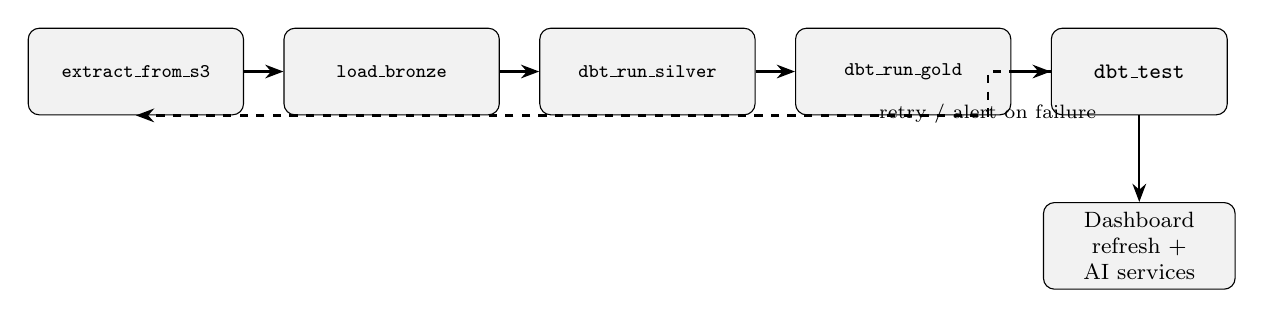
\begin{tikzpicture}[node distance=0.5cm]
\node[block,text width=2.5cm,font=\scriptsize\ttfamily] (t1) {extract\_from\_s3};
\node[block,text width=2.5cm,font=\scriptsize\ttfamily,right=of t1] (t2) {load\_bronze};
\node[block,text width=2.5cm,font=\scriptsize\ttfamily,right=of t2] (t3) {dbt\_run\_silver};
\node[block,text width=2.5cm,font=\scriptsize\ttfamily,right=of t3] (t4) {dbt\_run\_gold};
\node[block,text width=2.0cm,right=of t4] (t5) {\texttt{dbt\_test}};
\node[block,text width=2.2cm,below=1.1cm of t5] (t6) {Dashboard refresh + AI services};
\draw[arrow] (t1) -- (t2);
\draw[arrow] (t2) -- (t3);
\draw[arrow] (t3) -- (t4);
\draw[arrow] (t4) -- (t5);
\draw[arrow] (t5) -- (t6);
\draw[darrow] (t5.west) -- ++(-0.8,0) |- (t1.south) node[pos=0.25,below]{\scriptsize retry / alert on failure};
\end{tikzpicture}}
\caption{Implementation architecture and data flow realised by the Airflow DAG}
\label{fig:flow}
\end{figure}

\section{Technology Stack}
Table~\ref{tab:stack} lists the software components used in the implementation. Exact versions and configurations are recorded in Appendix~A.

\begin{table}[htbp]
\centering
\caption{Software components used in the prototype}
\label{tab:stack}
\small
\begin{tabular}{@{}p{3.2cm}p{6.2cm}p{3.6cm}@{}}
\toprule
\textbf{Component} & \textbf{Purpose} & \textbf{Version} \\
\midrule
Python with Pandas & Data handling and preparation scripts & \ph{record version} \\
Amazon S3 & Raw-file landing zone & Managed service \\
Snowflake & Analytical warehouse and layered storage & \ph{record version} \\
dbt Core & SQL transformations and data-quality tests & \ph{record version} \\
Apache Airflow & DAG-based scheduling and coordination & \ph{record version} \\
Snowflake Connector & Programmatic warehouse access & \ph{record version} \\
Streamlit & Web interface for dashboards and AI features & \ph{record version} \\
Grok API (xAI) & Review analysis and SQL generation & \ph{record model id} \\
\bottomrule
\end{tabular}
\end{table}

\section{Database Design}
The Gold layer uses a star-schema design. Table~\ref{tab:schema} summarises the principal tables and fields.

\begin{table}[htbp]
\centering
\caption{Gold-layer database schema (principal tables)}
\label{tab:schema}
\small
\begin{tabular}{@{}p{3.0cm}p{3.6cm}p{2.3cm}p{3.7cm}@{}}
\toprule
\textbf{Table} & \textbf{Column} & \textbf{Type} & \textbf{Description} \\
\midrule
\texttt{fact\_orders} & \texttt{order\_id} & VARCHAR & Order identifier (primary key) \\
 & \texttt{customer\_id} & VARCHAR & Customer foreign key \\
 & \texttt{restaurant\_id} & VARCHAR & Restaurant foreign key \\
 & \texttt{order\_ts} & TIMESTAMP & Order time \\
 & \texttt{delivery\_minutes} & NUMBER & Delivery duration \\
 & \texttt{total\_amount} & NUMBER & Order value \\
\midrule
\texttt{dim\_customers} & \texttt{customer\_id}, \texttt{city}, \texttt{signup\_date} & VARCHAR / DATE & Customer attributes \\
\midrule
\texttt{dim\_restaurants} & \texttt{restaurant\_id}, \texttt{cuisine}, \texttt{city}, \texttt{rating} & VARCHAR / NUMBER & Restaurant attributes \\
\midrule
\texttt{dim\_menu\_items} & \texttt{item\_id}, \texttt{restaurant\_id}, \texttt{price} & VARCHAR / NUMBER & Menu catalogue \\
\midrule
\texttt{stg\_reviews} & \texttt{review\_id}, \texttt{order\_id}, \texttt{rating}, \texttt{review\_text} & VARCHAR / NUMBER & Cleaned review records \\
\bottomrule
\end{tabular}
\end{table}

\section{Workflow Orchestration Design}
The Airflow DAG is configured with task-level retries and explicit dependencies, so that transformation tasks depend on successful loads, tests depend on transformations, and downstream refreshes depend on passing tests. Failures raise alerts instead of publishing outputs. Scheduling frequency is set for batch operation; near-real-time ingestion is left to future work.

\section{Review Analysis Module}
The review interface retrieves review records from Snowflake, selects a bounded sample of reviews per request, and sends the review text together with the user's instruction to the Grok API. The prompt requests concise summaries, recurring complaints, positive themes or grounded explanations, and instructs the model to use only the supplied text. The number of reviews per request, the truncation policy, the exact model identifier and the sampling method are documented in Appendix~A. Responses are displayed in Streamlit as model-generated analysis; they are not treated as validated sentiment classifications, and personally identifying content is filtered before any text is sent to the external API.

\section{Natural-Language-to-SQL Module}
For structured business questions, the application supplies the model with a description of approved tables and columns and requests SQL in a predictable response format. The generated query is checked against a keyword-level rule set (for example, rejecting statements that do not begin with \texttt{SELECT} and rejecting DDL or DML keywords), then executed through a read-only Snowflake role restricted to approved views, with query timeouts and row limits. Results are displayed as a table and, where appropriate, as a simple chart. Figure~\ref{fig:t2s} shows the intended interaction.

\begin{figure}[htbp]
\centering
\fbox{\parbox[c][5.5cm][c]{0.85\textwidth}{\centering\itshape
[PLACEHOLDER: Insert the actual screenshot showing a natural-language business question,\\
the generated SQL statement, and the returned result table or chart.]
}}
\caption{Natural-language-to-SQL interaction in the Streamlit interface (screenshot to be inserted)}
\label{fig:t2s}
\end{figure}

The keyword check is a preliminary safeguard, not a complete SQL parser or a substitute for database permissions; least-privilege roles remain the primary control.

\section{User Interface}
Streamlit provides the interface for the prototype. It brings together summary cards, time-series and category charts, result tables, the Text-to-SQL query form and the review-analysis interaction. Figure~\ref{fig:dash} shows the intended dashboard layout.

\begin{figure}[htbp]
\centering
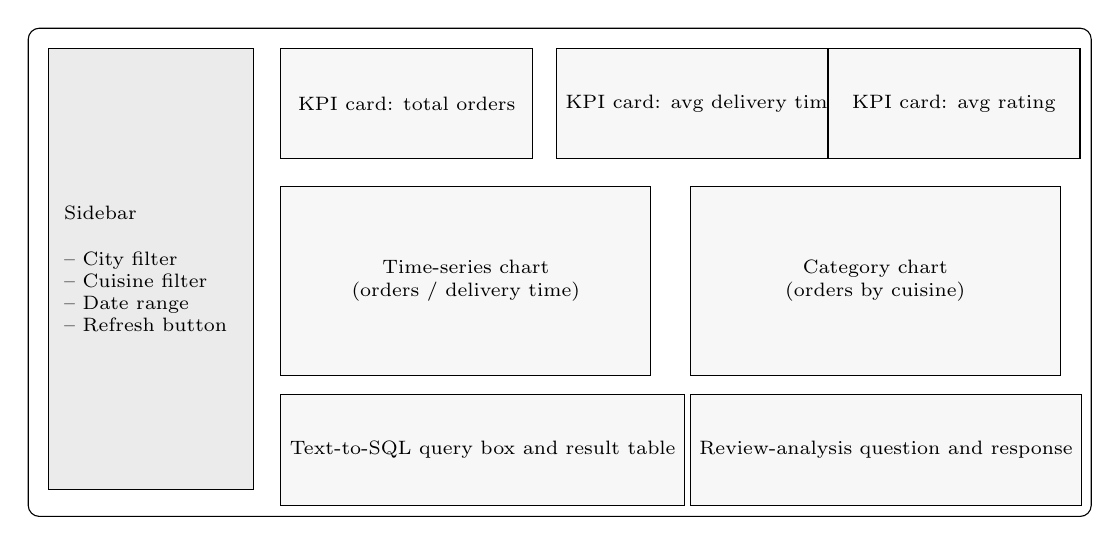
\begin{tikzpicture}
\draw[rounded corners] (0,0) rectangle (13.5,6.2);
\node[draw,fill=black!8,minimum width=2.6cm,minimum height=5.6cm,anchor=north west,text width=2.2cm,font=\scriptsize,align=left] at (0.25,5.95) {Sidebar\\[0.3cm] -- City filter\\ -- Cuisine filter\\ -- Date range\\ -- Refresh button};
\node[draw,fill=black!3,minimum width=3.2cm,minimum height=1.4cm,anchor=north west,font=\scriptsize] at (3.2,5.95) {KPI card: total orders};
\node[draw,fill=black!3,minimum width=3.2cm,minimum height=1.4cm,anchor=north west,font=\scriptsize] at (6.7,5.95) {KPI card: avg delivery time};
\node[draw,fill=black!3,minimum width=3.2cm,minimum height=1.4cm,anchor=north west,font=\scriptsize] at (10.15,5.95) {KPI card: avg rating};
\node[draw,fill=black!3,minimum width=4.7cm,minimum height=2.4cm,anchor=north west,font=\scriptsize,align=center] at (3.2,4.2) {Time-series chart\\(orders / delivery time)};
\node[draw,fill=black!3,minimum width=4.7cm,minimum height=2.4cm,anchor=north west,font=\scriptsize,align=center] at (8.4,4.2) {Category chart\\(orders by cuisine)};
\node[draw,fill=black!3,minimum width=4.7cm,minimum height=1.4cm,anchor=north west,font=\scriptsize,align=center] at (3.2,1.55) {Text-to-SQL query box and result table};
\node[draw,fill=black!3,minimum width=4.7cm,minimum height=1.4cm,anchor=north west,font=\scriptsize,align=center] at (8.4,1.55) {Review-analysis question and response};
\end{tikzpicture}
\caption{Dashboard layout of the Streamlit interface}
\label{fig:dash}
\end{figure}

\section{Implementation Workflow}
The implementation was carried out in the following sequence:
\begin{enumerate}[leftmargin=2em]
\item Prepare source files for customers, restaurants, menu items, orders, order items and reviews.
\item Upload the raw files to Amazon S3 and load them into Snowflake, retaining the raw representation in the Bronze layer.
\item Run dbt models to clean fields, standardise formats and build Silver tables.
\item Build Gold-level dimensions, facts and business marts for reporting.
\item Run dbt data-quality tests and check pipeline status.
\item Use Airflow to coordinate the sequence and schedule repeat runs.
\item Connect approved analytical tables to the Streamlit dashboard and the Text-to-SQL interface.
\item Send selected review text and the user's request to the Grok API and display the generated response.
\item Evaluate the system using the predefined functional and qualitative criteria.
\end{enumerate}

% =====================================================================
% CHAPTER 5: RESULTS AND DISCUSSION
% =====================================================================
\chaptersplit{5}{RESULTS AND DISCUSSION}

\chapter{RESULTS AND DISCUSSION}

\noindent This chapter reports what was observed during implementation and testing. Because measured results were not available when this draft was prepared, the tables below define the exact quantities to be recorded from actual runs; placeholders are marked and no unmeasured values are presented as final.

\section{Experimental Setup}
The evaluation uses the food-delivery dataset described in Chapter~4. Dataset size, row counts by table, Snowflake warehouse size, dbt and Airflow versions, execution environment and experimental duration are listed in Table~\ref{tab:pipeline}. Testing follows a fixed procedure: (i) each functional task is executed end to end and its outcome recorded; (ii) dbt test results are collected; (iii) a fixed set of business questions is asked through Text-to-SQL and each generated query is compared with a manually verified expected answer; and (iv) a fixed set of review questions is asked and each answer is inspected for relevance and support by the supplied reviews.

\section{Functional Results}
Table~\ref{tab:functional} records whether the system can complete each major task.

\begin{table}[htbp]
\centering
\caption{Functional test results (outcomes to be recorded from actual runs)}
\label{tab:functional}
\small
\begin{tabular}{@{}p{1.3cm}p{4.3cm}p{4.4cm}p{2.8cm}@{}}
\toprule
\textbf{Test ID} & \textbf{Feature tested} & \textbf{Expected result} & \textbf{Status} \\
\midrule
FT-01 & Upload and load dataset into Snowflake Bronze & All six tables loaded with expected row counts & \ph{record} \\
FT-02 & Build Silver models via dbt & Cleaned tables created without test failures & \ph{record} \\
FT-03 & Build Gold dimensions, facts and marts & Marts queryable by the dashboard & \ph{record} \\
FT-04 & Execute dbt data-quality tests & All configured tests pass & \ph{record} \\
FT-05 & Run the Airflow DAG end to end & DAG completes with all tasks successful & \ph{record} \\
FT-06 & Answer review prompts through the Grok API & Relevant, grounded answers displayed & \ph{record} \\
FT-07 & Execute approved Text-to-SQL queries & Correct result returned for verified questions & \ph{record} \\
\bottomrule
\end{tabular}
\end{table}

\section{Pipeline and Data-Quality Results}
Table~\ref{tab:pipeline} records records loaded per table, dbt tests passed and failed, and any errors found during testing. If incremental processing is implemented, the handling of new or changed records is documented in the notes column.

\begin{table}[htbp]
\centering
\caption{Dataset and pipeline summary (values to be recorded from actual runs)}
\label{tab:pipeline}
\small
\setlength{\tabcolsep}{4pt}
\begin{tabular}{@{}p{2.7cm}p{2.2cm}p{2.2cm}p{1.9cm}p{1.9cm}p{2.5cm}@{}}
\toprule
\textbf{Table / layer} & \textbf{Input rows} & \textbf{Output rows} & \textbf{Tests passed} & \textbf{Tests failed} & \textbf{Notes} \\
\midrule
Bronze (raw) & \ph{record} & \ph{record} & --- & --- & Raw copy retained \\
Silver (cleaned) & \ph{record} & \ph{record} & \ph{record} & \ph{record} & Type and null fixes \\
Gold: \texttt{fact\_orders} & \ph{record} & \ph{record} & \ph{record} & \ph{record} & Star schema \\
Gold: dimensions & \ph{record} & \ph{record} & \ph{record} & \ph{record} & Conformed keys \\
Reviews (staging) & \ph{record} & \ph{record} & \ph{record} & \ph{record} & Text cleaned \\
\bottomrule
\end{tabular}
\end{table}

\section{AI Interaction Results}
For the review feature, a fixed set of representative questions is used and both prompts and outputs are saved. A qualitative review records whether each answer is relevant to the supplied text, includes unsupported claims, or omits important evidence. These observations are not accuracy scores and are not generalised to all reviews.

For Text-to-SQL, business questions whose correct answers can be independently checked are used. Table~\ref{tab:ai} logs whether the generated SQL executes, uses approved tables and returns the expected result. Latency or API cost, if reported, is measured consistently with the stated test conditions.

\begin{table}[htbp]
\centering
\caption{AI feature test log (outcomes to be recorded from actual runs)}
\label{tab:ai}
\small
\begin{tabular}{@{}p{1.2cm}p{2.4cm}p{4.4cm}p{3.2cm}p{2.0cm}@{}}
\toprule
\textbf{ID} & \textbf{Feature} & \textbf{Question / input} & \textbf{Expected behaviour} & \textbf{Status} \\
\midrule
AI-01 & Review analysis & ``What are the most recurring delivery complaints?'' & Themes supported by supplied reviews & \ph{record} \\
AI-02 & Review analysis & ``Summarise positive feedback about food quality.'' & Grounded summary, no invented claims & \ph{record} \\
AI-03 & Text-to-SQL & ``Which city has the highest average order value?'' & Correct city with executed query & \ph{record} \\
AI-04 & Text-to-SQL & ``List the top five restaurants by average rating (min.\ 50 orders).'' & Correct ranking with join on approved marts & \ph{record} \\
\bottomrule
\end{tabular}
\end{table}

\section{Discussion}
The results must distinguish successful execution from answer quality. A pipeline can run successfully while still containing data-quality problems, and a query can execute without answering the user's question correctly. Likewise, a fluent review summary is not proof of sentiment-classification accuracy, nor is a sample of reviews statistically representative of all customers unless the sampling procedure supports that interpretation.

Observed failures are analysed together with their likely causes: for example, incorrect joins in generated SQL usually indicate that the schema description given to the model was incomplete, while unsupported claims in review answers usually indicate that the supplied context was too large or too loosely sampled. Changes made in response to such findings are recorded in Appendix~A. Where lower latency is reported, it is interpreted together with answer quality rather than in isolation.

\section{Limitations}
The following limitations apply to the current version:
\begin{itemize}[leftmargin=2em]
\item The evaluation dataset is of restricted size and covers a single domain and season of data; results may not generalise.
\item The review module uses direct prompting and is bounded by context length; it does not scale to very large review collections.
\item Review output is not a validated sentiment classifier and carries no measured accuracy claim.
\item The keyword-based SQL guard is a preliminary safeguard; unsafe patterns could in principle slip through or harmless queries be rejected.
\item The system is batch-oriented; no streaming ingestion or production availability is claimed.
\item External API usage incurs cost and rate limits, and only data permitted for external processing may be sent.
\end{itemize}

% =====================================================================
% CHAPTER 6: CONCLUSION AND FUTURE SCOPE
% =====================================================================
\chaptersplit{6}{CONCLUSION AND FUTURE SCOPE}

\chapter{CONCLUSION AND FUTURE SCOPE}

\section{Conclusion}
This project demonstrated a structured approach for developing a cloud-based food-delivery analytics prototype that combines data engineering with AI-assisted access to business information and customer feedback. Amazon S3 is used for raw-file storage, Snowflake for layered analytical storage and processing, dbt for declarative transformations and data-quality checks, Airflow for workflow orchestration, and Streamlit for the user interface.

The work addresses the objectives stated in Chapter~1. The pipeline ingests six domain tables and organises them into Bronze, Silver and Gold layers; dbt tests provide automated quality checks; Airflow coordinates repeatable runs; the Grok-based feature accepts review text and user instructions to produce summaries and observations; and the Text-to-SQL feature translates business questions into guarded, read-only queries over curated analytical tables. Keeping the review path and the query path separate makes their evidence sources and limitations explicit. The value of the project is the integration of these components into one workflow, together with an evaluation methodology that records functional outcomes, test results and qualitative observations honestly. The strength of the final system should be judged from the documented results once the placeholders in Chapter~5 are replaced with measured values.

\section{Future Scope}
The current implementation is a batch-oriented prototype. The following extensions are proposed, to be introduced based on demonstrated needs and tested individually:
\begin{itemize}[leftmargin=2em]
\item Stronger SQL validation: replace keyword checks with SQL parsing, allow-list validation and strict database permissions.
\item Review retrieval for larger datasets: add an embedding-based retrieval layer and evaluate it separately before describing the feature as retrieval-augmented.
\item Human-reviewed evaluation sets for review answers and SQL questions, enabling quantitative evaluation of relevance and correctness.
\item Operational monitoring of pipeline failures, API errors, query latency, token usage and estimated cost.
\item Incremental refresh and scheduling so that only new or changed records are processed.
\item Near-real-time ingestion and streaming updates for time-sensitive metrics.
\item Broader analytics, such as trends by city, cuisine, delivery-time band and review topic, and studies of whether delivery-time shifts associate with review sentiment.
\item Deployment hardening: access control, secrets management, logging, privacy checks and governance suitable for a larger user base.
\item Generalisation of the architecture to adjacent domains such as e-commerce and hospitality.
\end{itemize}

% =====================================================================
% REFERENCES
% =====================================================================
\clearpage
\addcontentsline{toc}{chapter}{REFERENCES}
\begin{thebibliography}{24}
\small

\bibitem{ref1} J. Schneider, C. Gr\"oger, A. Lutsch, H. Schwarz, and B. Mitschang, ``The lakehouse: State of the art on concepts and technologies,'' \emph{SN Comput. Sci.}, vol. 5, no. 4, Art. no. 449, 2024, doi: 10.1007/s42979-024-02737-0.

\bibitem{ref2} A. Mbata, Y. Sripada, and M. Zhong, ``A survey of pipeline tools for data engineering,'' \emph{arXiv:2406.08335}, 2024.

\bibitem{ref3} A. Vaswani \emph{et al.}, ``Attention is all you need,'' in \emph{Proc. NeurIPS}, 2017, \emph{arXiv:1706.03762}.

\bibitem{ref4} T. B. Brown \emph{et al.}, ``Language models are few-shot learners,'' in \emph{Proc. NeurIPS}, 2020.

\bibitem{ref5} P. Lewis \emph{et al.}, ``Retrieval-augmented generation for knowledge-intensive NLP tasks,'' in \emph{Proc. NeurIPS}, 2020, \emph{arXiv:2005.11401}.

\bibitem{ref6} T. Yu \emph{et al.}, ``Spider: A large-scale human-labeled dataset for complex and cross-domain semantic parsing and text-to-SQL task,'' in \emph{Proc. EMNLP}, 2018, pp. 3911--3921, doi: 10.18653/v1/D18-1425.

\bibitem{ref7} M. Armbrust \emph{et al.}, ``Lakehouse: A new generation of open platforms that unify data warehousing and advanced analytics,'' in \emph{Proc. CIDR}, 2021.

\bibitem{ref8} M. Armbrust \emph{et al.}, ``Delta Lake: High-performance ACID table storage over cloud object stores,'' \emph{Proc. VLDB Endow.}, vol. 13, no. 12, pp. 1687--1692, 2020.

\bibitem{ref9} N. Polyzotis, S. Karampatzakis, A. Kumar, and A. Tsoumakas, ``Data management challenges in production machine learning,'' in \emph{Proc. ACM SIGMOD}, 2017, pp. 1721--1734.

\bibitem{ref10} S. Gupta, R. Ranjan, and S. N. Singh, ``A comprehensive survey of retrieval-augmented generation (RAG): Evolution, current landscape and future directions,'' \emph{arXiv:2410.12837}, 2024, doi: 10.48550/arXiv.2410.12837.

\bibitem{ref11} A. Branco, D. Parada, M. Silva, F. Mendon\c{c}a, S. S. Mostafa, and F. Morgado-Dias, ``Sentiment analysis in Portuguese restaurant reviews: Application of transformer models in edge computing,'' \emph{Electronics}, vol. 13, no. 3, Art. no. 589, 2024, doi: 10.3390/electronics13030589.

\bibitem{ref12} J. Devlin, M.-W. Chang, K. Lee, and K. Toutanova, ``BERT: Pre-training of deep bidirectional transformers for language understanding,'' in \emph{Proc. NAACL-HLT}, 2019, pp. 4171--4186.

\bibitem{ref13} L. Zhao \emph{et al.}, ``A survey for large language models,'' \emph{arXiv:2303.18223}, 2023.

\bibitem{ref14} J. Li \emph{et al.}, ``Can LLM already serve as a database interface? A BIg bench for large-scale database grounded text-to-SQLs,'' in \emph{Proc. NeurIPS}, 2023.

\bibitem{ref15} S. Talaei, M. Pourreza, Y.-C. Chang, A. Mirhoseini, and A. Saberi, ``CHESS: Contextual harnessing for efficient SQL synthesis,'' \emph{arXiv:2405.16755}, 2024.

\bibitem{ref16} V. Zhong, C. Xiong, and R. Socher, ``Seq2SQL: Generating structured queries from natural language using reinforcement learning,'' in \emph{Proc. ACL}, 2017.

\bibitem{ref17} Y. Chang \emph{et al.}, ``TAPEX: Table pre-training via learning a neural SQL solver,'' in \emph{Proc. ACL}, 2022, pp. 53--65.

\bibitem{ref18} Apache Software Foundation, ``Apache Airflow documentation: What is Airflow?'' [Online]. Available: https://airflow.apache.org/docs/. Accessed: Sep. 18, 2026.

\bibitem{ref19} dbt Labs, ``dbt documentation.'' [Online]. Available: https://docs.getdbt.com/. Accessed: Sep. 18, 2026.

\bibitem{ref20} Amazon Web Services, ``Amazon S3 documentation.'' [Online]. Available: https://docs.aws.amazon.com/s3/. Accessed: Sep. 18, 2026.

\bibitem{ref21} Snowflake Inc., ``Snowflake documentation.'' [Online]. Available: https://docs.snowflake.com/. Accessed: Sep. 18, 2026.

\bibitem{ref22} Streamlit, ``Streamlit documentation.'' [Online]. Available: https://docs.streamlit.io/. Accessed: Sep. 18, 2026.

\bibitem{ref23} xAI, ``xAI API documentation (Grok).'' [Online]. Available: https://docs.x.ai/. Accessed: Sep. 18, 2026.

\bibitem{ref24} W. McKinney, ``Data structures for statistical computing in Python,'' in \emph{Proc. 9th Python in Science Conf.}, 2010, pp. 56--61.

\end{thebibliography}

% =====================================================================
% APPENDIX A
% =====================================================================
\clearpage
\chapter*{APPENDIX A: IMPLEMENTATION CONFIGURATIONS AND PROMPT TEMPLATES}
\addcontentsline{toc}{chapter}{APPENDIX A}

\section{Environment Variables}
Credentials are supplied through environment variables and are never hard-coded in source files:
\begin{itemize}[leftmargin=2em]
\item Snowflake: \path{SNOWFLAKE_ACCOUNT}, \path{SNOWFLAKE_USER}, \path{SNOWFLAKE_PASSWORD}, \path{SNOWFLAKE_ROLE} (read-only role), \path{SNOWFLAKE_WAREHOUSE}, \path{SNOWFLAKE_DATABASE}, \path{SNOWFLAKE_SCHEMA}
\item AWS S3: \path{AWS_ACCESS_KEY_ID}, \path{AWS_SECRET_ACCESS_KEY}, \path{S3_BUCKET}
\item Grok API: \path{XAI_API_KEY}
\end{itemize}

\section{dbt Data-Quality Tests Configured}
\begin{itemize}[leftmargin=2em]
\item \texttt{unique} on primary keys of all dimension and fact tables.
\item \texttt{not\_null} on key, timestamp and monetary columns of \texttt{fact\_orders}.
\item \texttt{relationships} from fact foreign keys to dimension keys.
\item \texttt{accepted\_values} on categorical columns such as order status and cuisine.
\end{itemize}

\section{Review-Analysis Prompt Template}
\begin{quote}
\small\itshape You are an analytics assistant. Use ONLY the review text supplied below. Do not invent facts, ratings, or customer names that are not present in the text. If the reviews are insufficient, say so. Question: \{user\_question\} --- Reviews: \{review\_samples\}
\end{quote}

\section{SQL Guard Rules (Preliminary)}
\begin{itemize}[leftmargin=2em]
\item The statement must begin with \texttt{SELECT} (after trimming whitespace and comments).
\item Forbidden keywords: \texttt{INSERT}, \texttt{UPDATE}, \texttt{DELETE}, \texttt{DROP}, \texttt{ALTER}, \texttt{CREATE}, \texttt{TRUNCATE}, \texttt{GRANT}, \texttt{CALL}, \texttt{EXECUTE}.
\item Execution uses a read-only role limited to approved Gold views, with a statement timeout and a row limit.
\end{itemize}

\section{Recorded Versions}
\begin{center}
\begin{tabular}{@{}ll@{}}
\toprule
\textbf{Item} & \textbf{Value} \\
\midrule
Python / Pandas & \ph{record} \\
dbt Core & \ph{record} \\
Apache Airflow & \ph{record} \\
Snowflake account edition / warehouse size & \ph{record} \\
Grok model identifier & \ph{record} \\
Dataset source, licence, row counts, date range & \ph{record} \\
\bottomrule
\end{tabular}
\end{center}

% =====================================================================
% ANNEXURE A
% =====================================================================
\clearpage
\chapter*{ANNEXURE A: PUBLICATIONS AND INTELLECTUAL PROPERTY}
\addcontentsline{toc}{chapter}{ANNEXURE A}

\noindent This annexure records documentary evidence related to project outcomes, such as published or submitted papers, conference publications, patent applications, design registrations and other relevant intellectual property. The status of each item is clearly stated.

\begin{table}[htbp]
\centering
\caption{Annexure A: Publications and intellectual property}
\small
\begin{tabular}{@{}p{2.6cm}p{7.2cm}p{2.8cm}@{}}
\toprule
\textbf{Type} & \textbf{Title / description} & \textbf{Status} \\
\midrule
Research paper & ``An Integrated Cloud Data Engineering and AI Analytics Platform for Food-Delivery Data'' (A.\ Saw, A.\ Kolhe, A.\ Paradkar) & Draft prepared; journal / conference submission planned \\
Patent / design & --- & None filed \\
Copyright / dataset & Project source code repository & To be registered on publication of the repository \\
\bottomrule
\end{tabular}
\end{table}

% =====================================================================
% ANNEXURE B
% =====================================================================
\clearpage
\chapter*{ANNEXURE B: STUDENT CONTRIBUTION STATEMENT}
\addcontentsline{toc}{chapter}{ANNEXURE B}

\noindent For group projects, each student specifies a specific and verifiable contribution. The split below reflects the division of work carried out for this project and may be revised by the team to match the final division of labour.

\begin{table}[htbp]
\centering
\caption{Annexure B: Student contribution statement}
\small
\begin{tabular}{@{}p{3.0cm}p{3.2cm}p{6.4cm}@{}}
\toprule
\textbf{Student name} & \textbf{Roll number} & \textbf{Contribution} \\
\midrule
Amit Saw & \ph{roll number} & Literature review, dataset collection, S3 and Bronze-layer ingestion setup \\
Ankit Kolhe & \ph{roll number} & Snowflake modelling, dbt transformations and tests, Airflow DAG design \\
Aryan Paradkar & \ph{roll number} & Streamlit interface, Grok review module, Text-to-SQL module, testing and documentation \\
\bottomrule
\end{tabular}
\end{table}

% =====================================================================
% ANNEXURE C
% =====================================================================
\clearpage
\chapter*{ANNEXURE C: PROJECT OUTPUTS}
\addcontentsline{toc}{chapter}{ANNEXURE C}

\noindent Major outputs generated from the project are listed below:
\begin{itemize}[leftmargin=2em]
\item \textbf{Working prototype:} cloud pipeline (S3, Snowflake, dbt, Airflow) with Streamlit interface --- \emph{implemented; screenshots to be attached}.
\item \textbf{Software / application:} Streamlit analytics application with dashboard, review analysis and Text-to-SQL modules --- \emph{implemented}.
\item \textbf{Dataset:} curated food-delivery dataset in Bronze, Silver and Gold layers --- \emph{loaded; row counts to be recorded}.
\item \textbf{Research publication:} draft research paper (Annexure A) --- \emph{in preparation}.
\item \textbf{GitHub / project repository:} source code, dbt models and Airflow DAG files --- \emph{to be uploaded}.
\item \textbf{Technology demonstration:} live demonstration of the dashboard, review analysis and natural-language querying --- \emph{scheduled with the project guide}.
\end{itemize}

\end{document}
